%----------------------------------------------------------------
%
%  File    :  survey-browsers.tex
%
%  Author  :  Keith Andrews, IICM, TU Graz, Austria
% 
%  Created :  27 May 1993
% 
%  Changed :  16 Nov 2010
% 
%----------------------------------------------------------------


\chapter{HTML Tables}

\label{HTML5 Tables}

In case of having much data to display, or data which is better of in a grid, HTML tables
are the best solution available. Before, tables have been used mostly for the layout of 
HTML web-sites and it is not a good practice to do so, mainly because of two things:
 

$\bullet$ Semantically it is wrong

$\bullet$ Tables aren't as adaptable and flexible as divs'

\section{Structure of tables}

The basic structure of an HTML table starts with the \textit{<table>} tag. It is the starting
point for constructing a table. Now, HTML tables consist of columns and rows, like normal
tables. For rows, the tag  \textit{<tr>} is used, whereas for table header \textit{<th>} tag
is used. Normally, table headers are positioned in the center and are bold. For table cells
\textit{<td>} tag is used [7]. 

\begin{lstlisting}[%
    language = CSS, 
    xleftmargin=0cm,              % no extra margins for floats
    xrightmargin=0cm,             % no extra margins for floats
    language=biblatex,
    basicstyle=\footnotesize\ttfamily,
    frame=shadowbox,
    numbers=left,
    label=list:BibACMIEEE,
    ,
]
    % An example of an HTML Table which demonstrates information about cars:
    <!DOCTYPE html>
<html>
<head>
	<title>Best Cars 2019</title>
</head>
<body>
<table class="table table-bordered table-hover table-condensed">
	<thead>
		<tr>
			<th title="Field #1">Car</th>
			<th title="Field #2">Manufacturer</th>
			<th title="Field #3">Engine Size</th>
			<th title="Field #4">Cylinders</th>
			<th title="Field #5">Horsepower</th>
			<th title="Field #6">Torque</th>
			<th title="Field #7">Compresion Ratio</th>
			<th title="Field #8">Miles per gallon</th>
			<th title="Field #9">Price</th>
		</tr>
	</thead>
	<tbody>
		<tr>
			<td>2019 Acura RDX</td>
			<td>Acura</td>
			<td>2.00L</td>
			<td align="right">4</td>
			<td align="right">272</td>
			<td align="right">280</td>
			<td>9.8:1</td>
			<td align="right">28</td>
			<td>€33,600.00</td>
		</tr>
		<tr>
			<td>2019 Ford Ranger</td>
			<td>Ford</td>
			<td>2.30L</td>
			<td align="right">4</td>
			<td align="right">270</td>
			<td align="right">310</td>
			<td>10.0:1</td>
			<td align="right">21</td>
			<td>€21,800.00</td>
		</tr>
	</tbody>
</table>

</body>
</html>
    
\end{lstlisting}

Now, there exist some other tags which can be used for HTML5 tables:

$\bullet$ <thead> - Table header, it is used to point out single or multiple rows 
of a table, which do not contain table data but column labels [8].

$\bullet$ <tbody> - Table body, it is used to point out <tr> elements. Position this tag
always after <thead>, but it can also come after or before <tfoot> [8].

$\bullet$ <tfoot> - Table footer, it is used to point out single or multiple <tr> elements
where those elements are presenting an overview  of the data in the table [8]. 

$\bullet$ <caption> - Table caption, as the name already says, can be used to specify table caption.
Can be put on the bottom of the CSS document.

$\bullet$ <col> - While using col and some other keyword, for example, align, it is possible direct
the alignment of text in the table. There are other keywords whom can be used to adjust colors, width
and many other things of table columns.  
 

\section{Responsive Tables}

Data tables can contain many information, which makes displaying that data quite messy and hard to
look at. So by using responsive design, a big favor is done to the clients,
by adjusting the table according to their devices. One idea would be to minimize the table, but if the user is looking
at the table from his mobile device, he would have to zoom in, which is not that useful to him, because then again he would need to scroll
to view the whole table [9].

\begin{figure}[H]
    \centering
  
    {%
    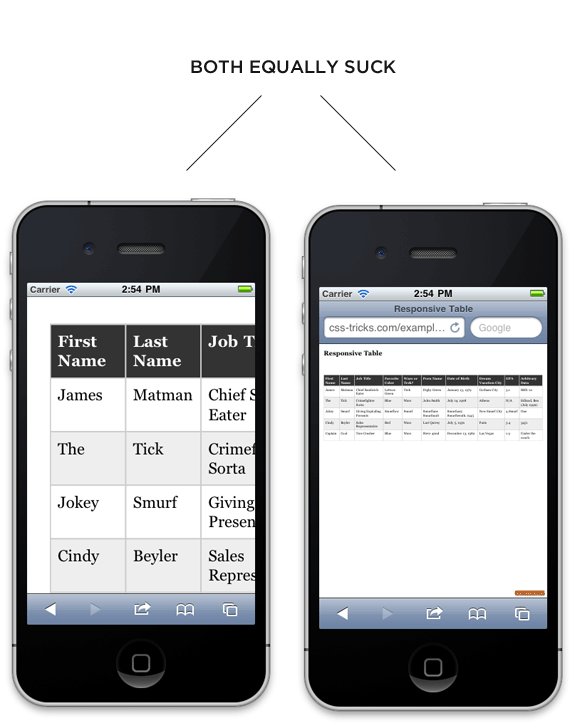
\includegraphics[width=\linewidth]
    {zoom_1.png}%
    \label{alig1}%
    }

    
    \caption[]
    {
      
    \imgcredit{https://css-tricks.com/responsive-data-tables/.}
    }
    \label{figWhol}
\end{figure}

As seen in the figure above, both options do not really look nor do as any good.
So, by using some simple CSS it is possible to fix that problem. With the help of the mentioned
media queries, it is possible to specify for which device sizes, which settings should be used. 

\begin{lstlisting}[%
    language = HTML, 
    xleftmargin=0cm,              % no extra margins for floats
    xrightmargin=0cm,             % no extra margins for floats
    language=biblatex,
    basicstyle=\footnotesize\ttfamily,
    frame=shadowbox,
    numbers=left,
    label=list:BibACMIEEE,
     stringstyle=\color{blue}
    ,
]
    % An example of using simple CSS with media queries on how to achieve Responsive Design:

    @media 
only screen and (max-width: 760px),
(min-device-width: 768px) and (max-device-width: 1024px)  {

	/* Force table to not be like tables anymore */
	table, thead, tbody, th, td, tr { 
		display: block; 
	}
	
	/* Hide table headers (but not display: none;, for accessibility) */
	thead tr { 
		position: absolute;
		top: -624.9375rem;
		left: -624.9375rem;
	}
	
	tr { border: 1px solid #ccc; }
	
	td { 
		/* Behave  like a "row" */
		border: none;
		border-bottom: 1px solid #eee; 
		position: relative;
		padding-left: 50%; 
	}
	
	td:before { 
		/* Now like a table header */
		position: absolute;
		/* Top/left values mimic padding */
		top: 0;
		left: 0.375rem;
		width: 45%;
		padding-right: 0.625rem;
		white-space: nowrap;
	}

\end{lstlisting}

\newpage
And now, the end result would be the following one:
\begin{figure}[H]
    \centering
  
    {%
    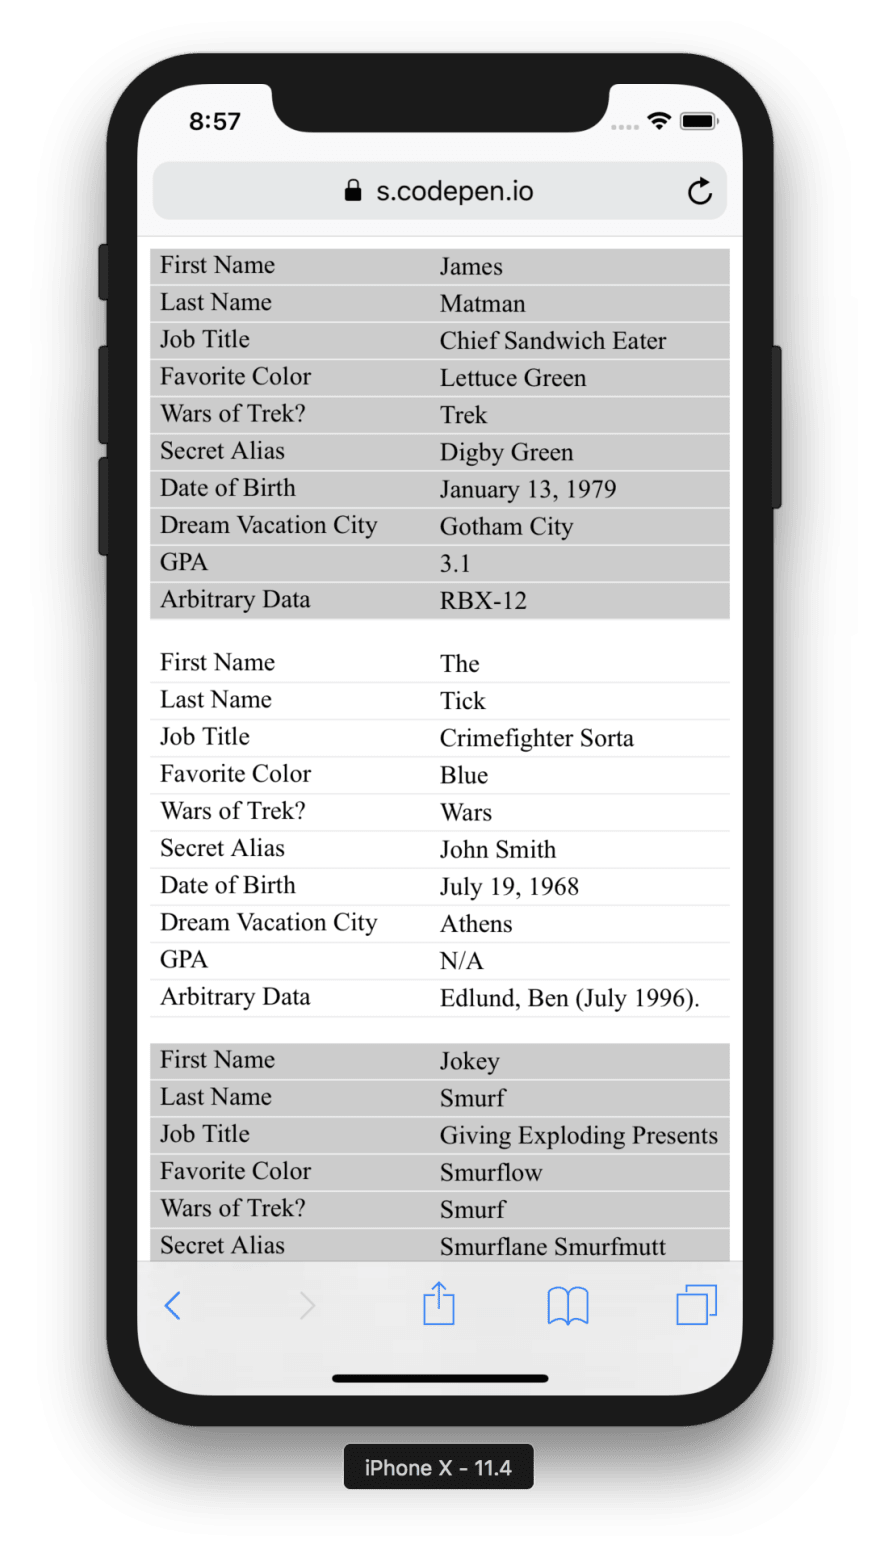
\includegraphics[width=0.45\linewidth]
    {zoom_3.png}%
    \label{alig1}%
    }

    
    \caption[Abstract Clock Towers]
    {
      
    \imgcredit{https://css-tricks.com/responsive-data-tables/.}
    }
    \label{figWhol}
\end{figure}


\section{Good Table Design}
Now, there are certain guidelines which can help a developer, or if that person can be called that way,
table maintainer, make a table and its design better. By that is meant that there are some interesting ways
where a little of simple CSS can be used to your advantage to make your table stand out.


\subsection{Alternate row highlighting}
When presented a table with a lot of entries, it can be hard to look at. Scrolling through numerous rows can be frustrating.
With this CSS trick, it can be a bit easier, atleast for the eyes if nothing else. The idea is to color every even row, while leaving
the odd ones in tact. 
As said, it is pretty simple, and requires only two lines of CSS, but also pretty useful.


\begin{lstlisting}[%
    language = HTML, 
    xleftmargin=0cm,              % no extra margins for floats
    xrightmargin=0cm,             % no extra margins for floats
    language=biblatex,
    basicstyle=\footnotesize\ttfamily,
    frame=shadowbox,
    numbers=left,
    label=list:BibACMIEEE,
     stringstyle=\color{blue}
    ,
]
    % An example of using simple CSS to color table rows:

	table.alt tr:nth-child(even) {background: #CCC}
	table.alt tr:nth-child(odd) {background: #FFF}

\end{lstlisting}

\newpage
And now, at the end, this is the final result:
\begin{figure}[H]
    \centering
  
    {%
    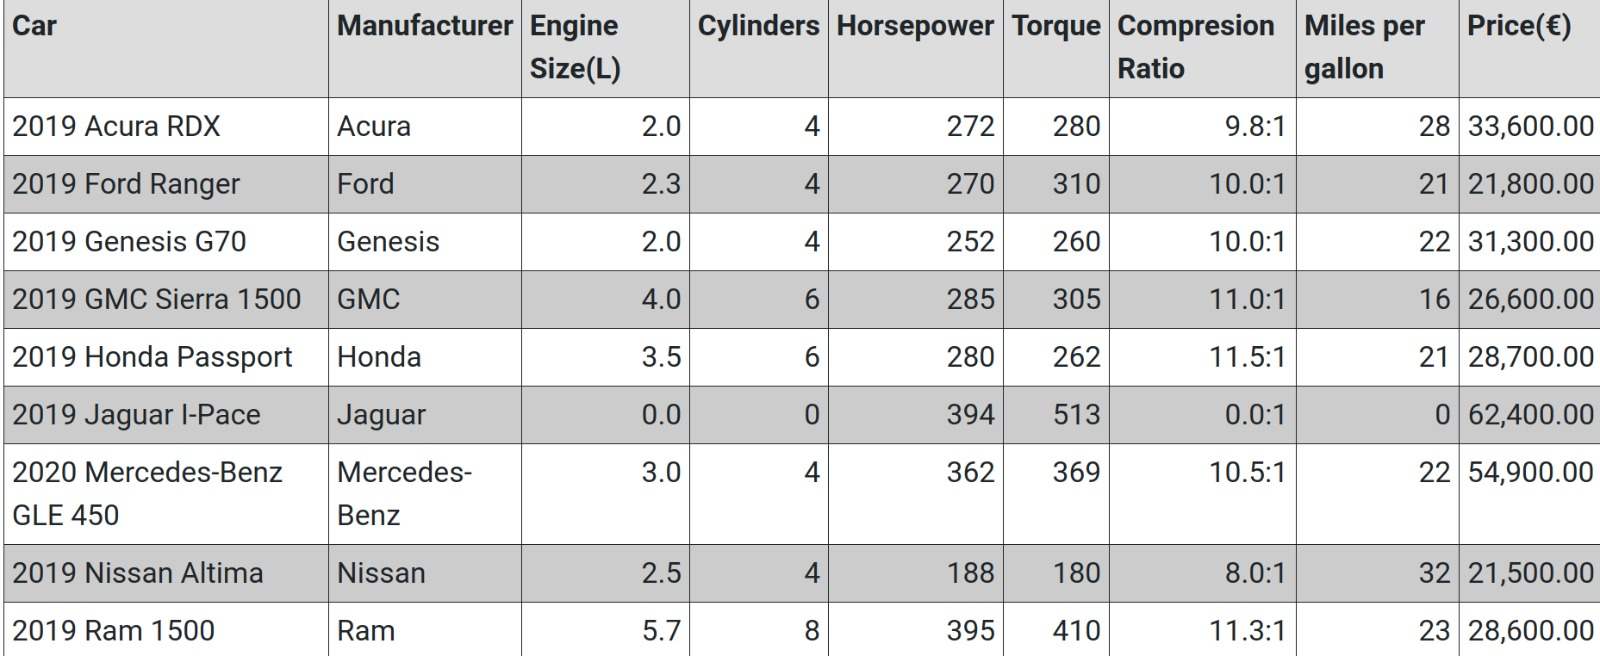
\includegraphics[width=\linewidth]
    {alt_t.jpeg}%
    \label{alig1}%
    }

    
    \caption[Abstract Clock Towers]
    {
      
    \imgcredit{Screenshot taken by the author.}
    }
    \label{figWhol}
\end{figure}


\subsection{Current Row Highlighting}
Now again, talking about a big table, and going through it, one may 
easily becomes lost and wouldn't know in which row he is at the moment, which can be
pretty stressful. Again with the help of some CSS, the lives of the users' is made easier.

\begin{lstlisting}[%
    language = HTML, 
    xleftmargin=0cm,              % no extra margins for floats
    xrightmargin=0cm,             % no extra margins for floats
    language=biblatex,
    basicstyle=\footnotesize\ttfamily,
    frame=shadowbox,
    numbers=left,
    label=list:BibACMIEEE,
     stringstyle=\color{blue}
    ,
]
    % An example of using simple CSS to highlight table rows:

	table {
      overflow: hidden;
	}

	tr:hover {
	  background-color: #ffa;
	}

	td, th {
	  position: relative;
	}
	td:hover::after,
	th:hover::after {
	  content: "";
	  position: absolute;
	  background-color: #ffa;
	  left: 0;
	  width: 100%;
	  z-index: -1;
	}

\end{lstlisting}


\newpage

And again, it is shown how a small amount of CSS can be helpful.
The result:
\begin{figure}[H]
    \centering
  
    {%
    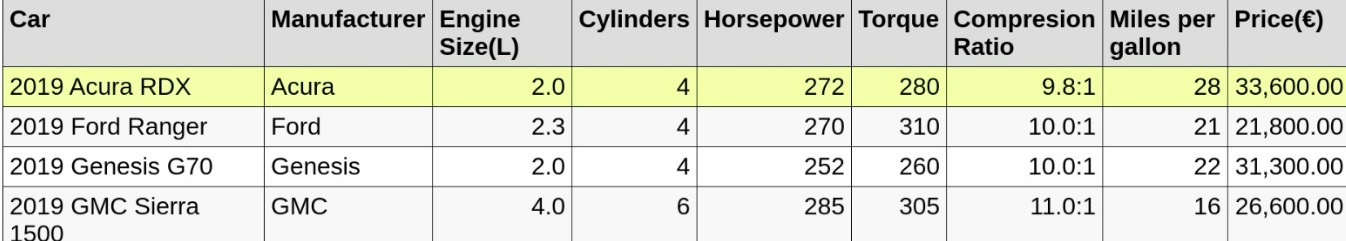
\includegraphics[width=\linewidth]
    {current_hl.jpeg}%
    \label{alig1}%
    }

    
    \caption[Abstract Clock Towers]
    {
      
    \imgcredit{Screenshot taken by the author.}
    }
    \label{figWhol}
\end{figure}


\subsection{Inclusive}

\subsection{Overlapping}






\section{Evaluating Hierarchy Browsers}

\subsection{Formative Studies}

\subsection{Comparative Studies}


